

\documentclass[11pt]{article}

\usepackage[T1]{fontenc}
\usepackage{lmodern}

\usepackage[margin=1in]{geometry}
\usepackage{graphicx}
\usepackage{float}
\usepackage{setspace}
\usepackage{caption}
\captionsetup{font=small, skip=6pt}

\title{A1: Workarounds}
\author{Alejandro De La Torre}
\date{\today}

\begin{document}
\maketitle
\onehalfspacing

\section{Overview}
This assignment documents three \emph{thoughtless acts}---everyday workarounds that reveal how people adapt environments not fully designed for their needs. Rather than focusing on intentional design or formal solutions, these observations highlight subtle, improvised actions that emerge naturally when objects or systems fall short. Across all three cases, individuals repurpose available resources to reduce friction, regain control, or complete a task more effectively.

\section{Consolidating Messy Food into a Single Bowl}
\begin{figure}[H]
    \centering
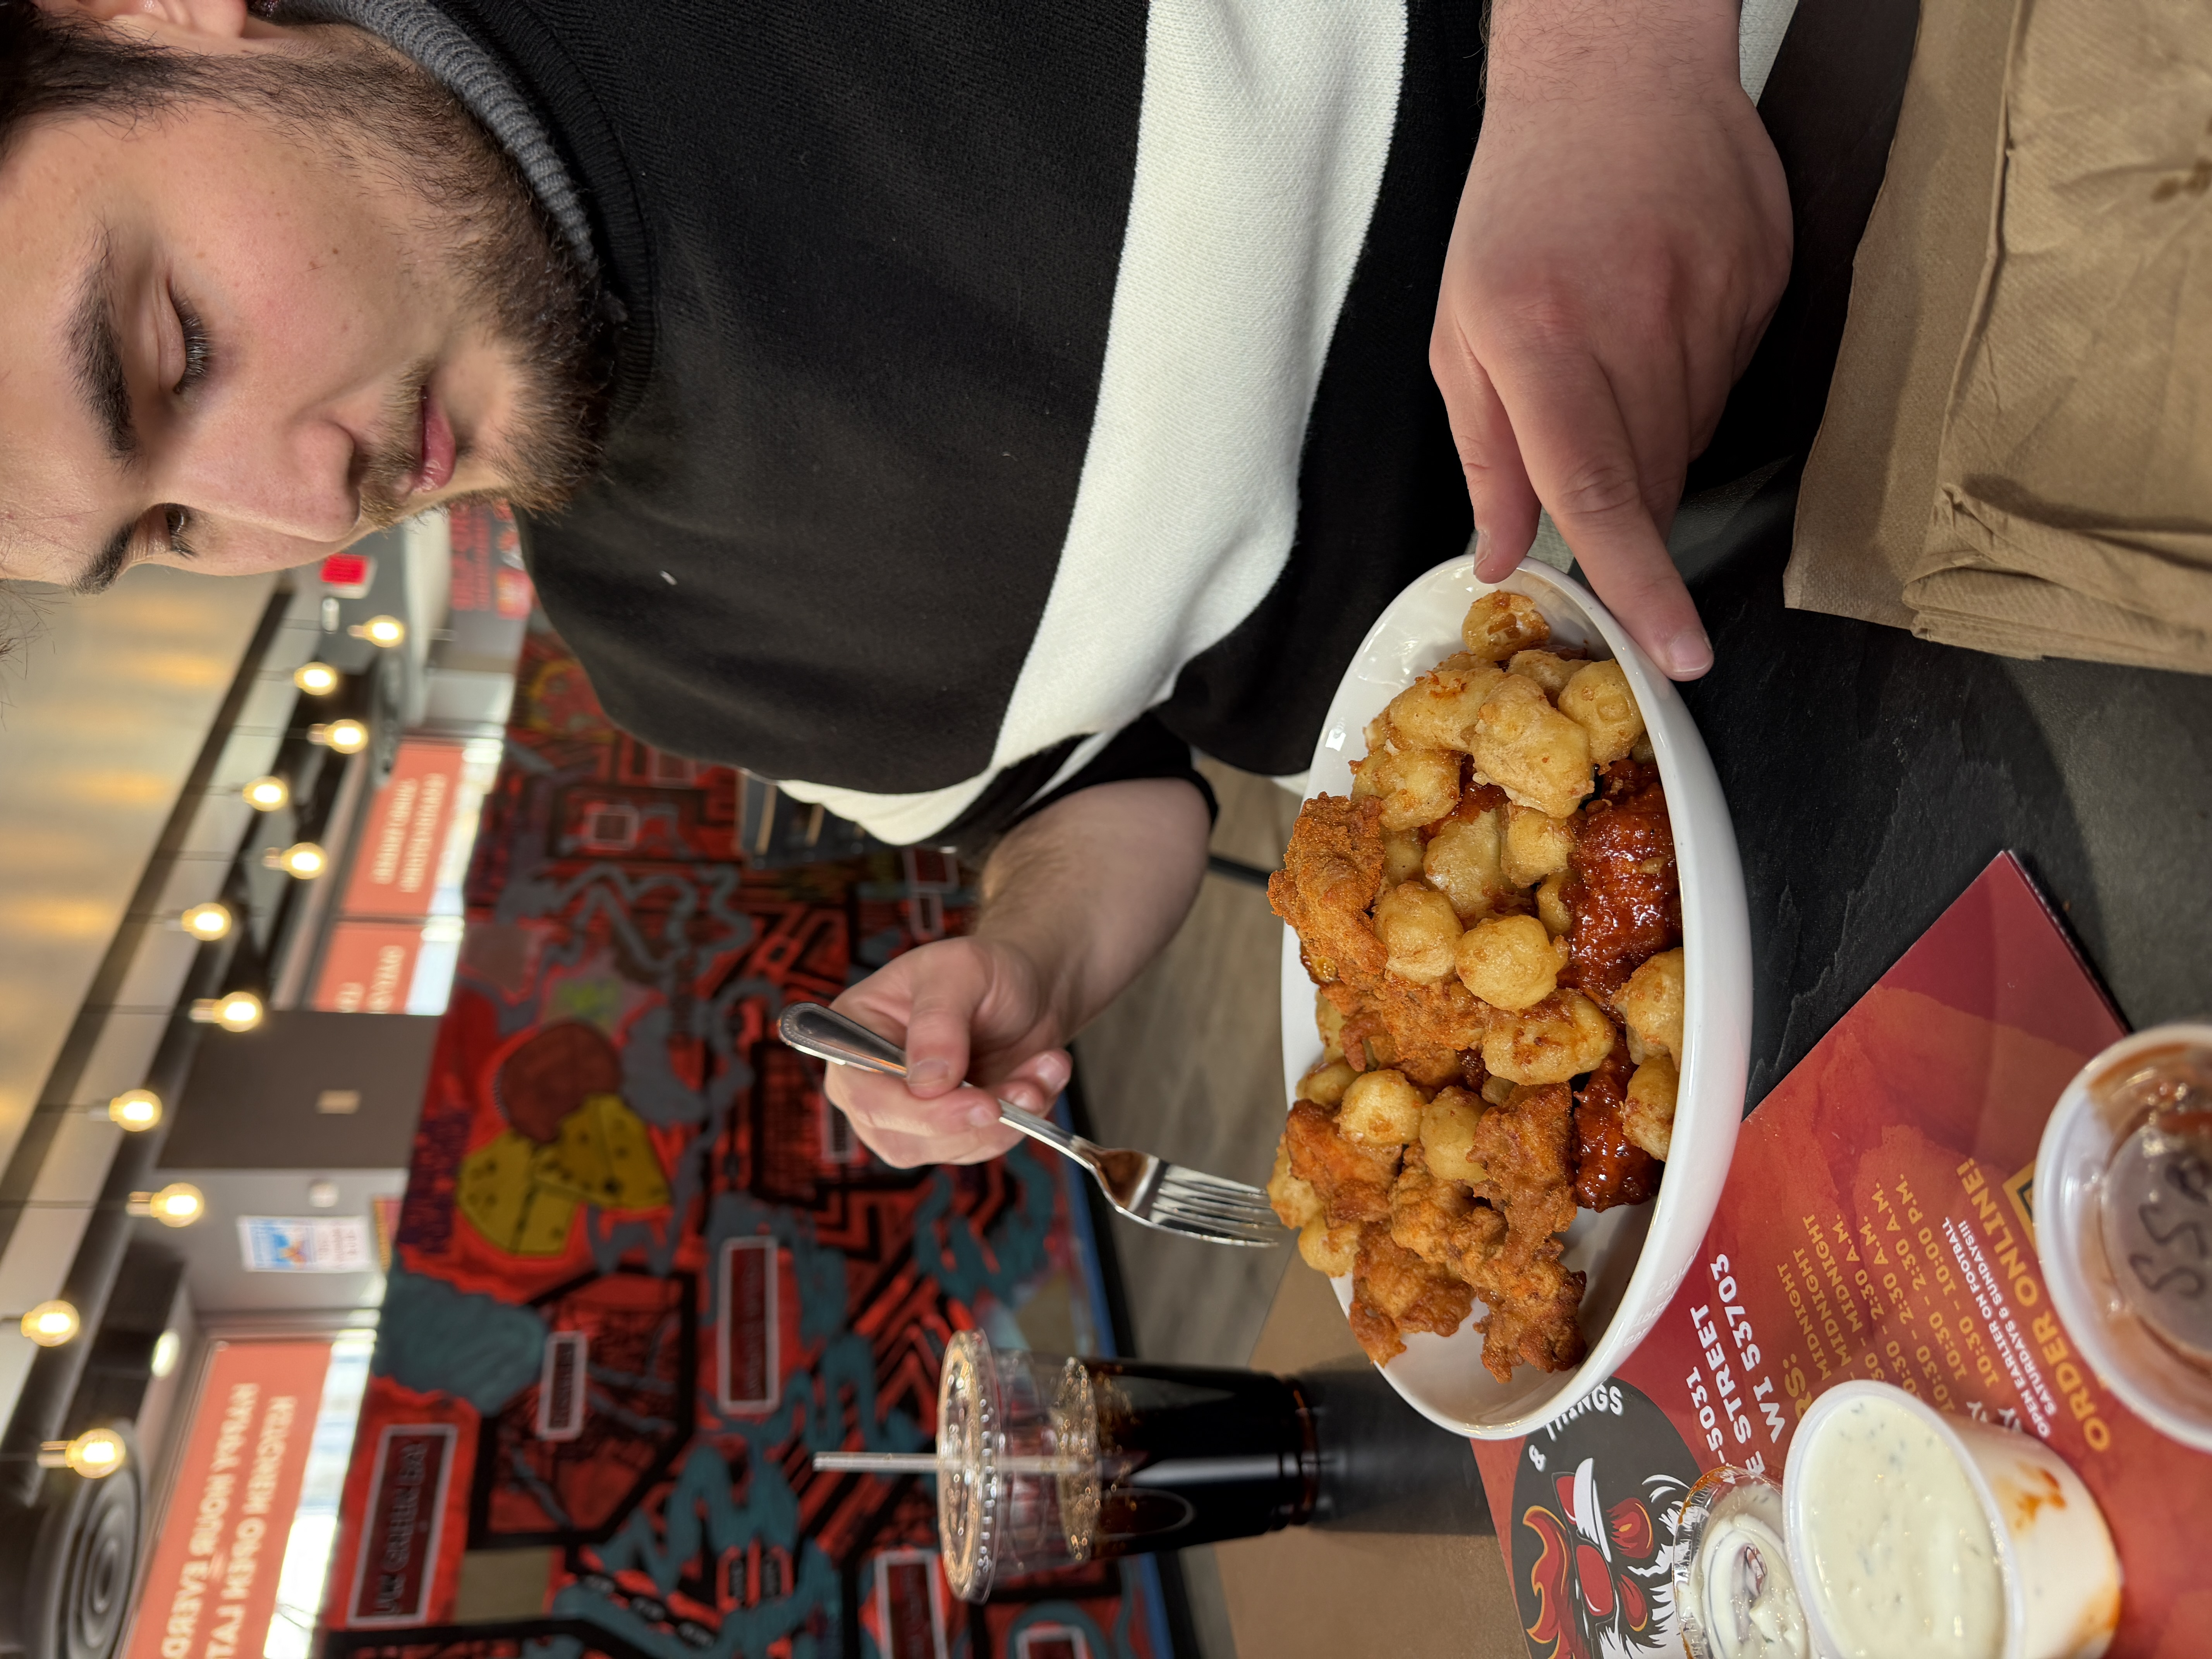
\includegraphics[angle=270, width=0.5\linewidth]{images/noah-nugs.JPG}
    \caption{Multiple messy food items consolidated into a single bowl to simplify eating and dipping.}
\end{figure}

This thoughtless act was observed at a casual restaurant while dining with a friend. The meal consisted of wings, nuggets, and sides, each served on separate plates alongside multiple dipping sauces. While visually abundant, this presentation made it difficult to eat efficiently without frequent plate switching, spills, or awkward hand movements.

The unmet need in this situation was the ability to eat a messy, multi-component meal in a controlled and efficient way. In response, the diner combined all food items into a single bowl, effectively transforming the meal into a contained mixture. This improvised solution centralized sauces, reduced the risk of spills, and allowed for one-handed eating at a comfortable pace.

By altering the format of the meal, the diner adapted the environment to better match their needs without modifying the food itself. This workaround illustrates how users quietly redesign experiences when presentation prioritizes abundance or aesthetics over usability.

\section{Removing a Tree Stump Using a Truck and Strap}
\begin{figure}[H]
    \centering
\includegraphics[width=0.6\linewidth]{images/tree-stump.JPG}
    \caption{A tree stump removed by attaching a strap to a pickup truck to generate pulling force.}
\end{figure}

This workaround was observed during a home yard project involving the removal of a large tree stump. Commercial stump-removal tools are often expensive, heavy, or inaccessible to homeowners, leaving a gap between professional equipment and household needs.

The unmet need was the ability to remove a deeply embedded stump using readily available resources. To address this, a strap was secured around the stump and attached to a pickup truck. The vehicle was then used to apply controlled pulling force until the stump loosened from the ground.

This solution leveraged an existing household asset to provide mechanical advantage typically supplied by specialized machinery. The act demonstrates how users creatively bridge gaps in tool availability by repurposing familiar objects for unintended but effective uses.

\section{Bathroom Floor Repair Through Improvised Tools}
\begin{figure}[H]
    \centering
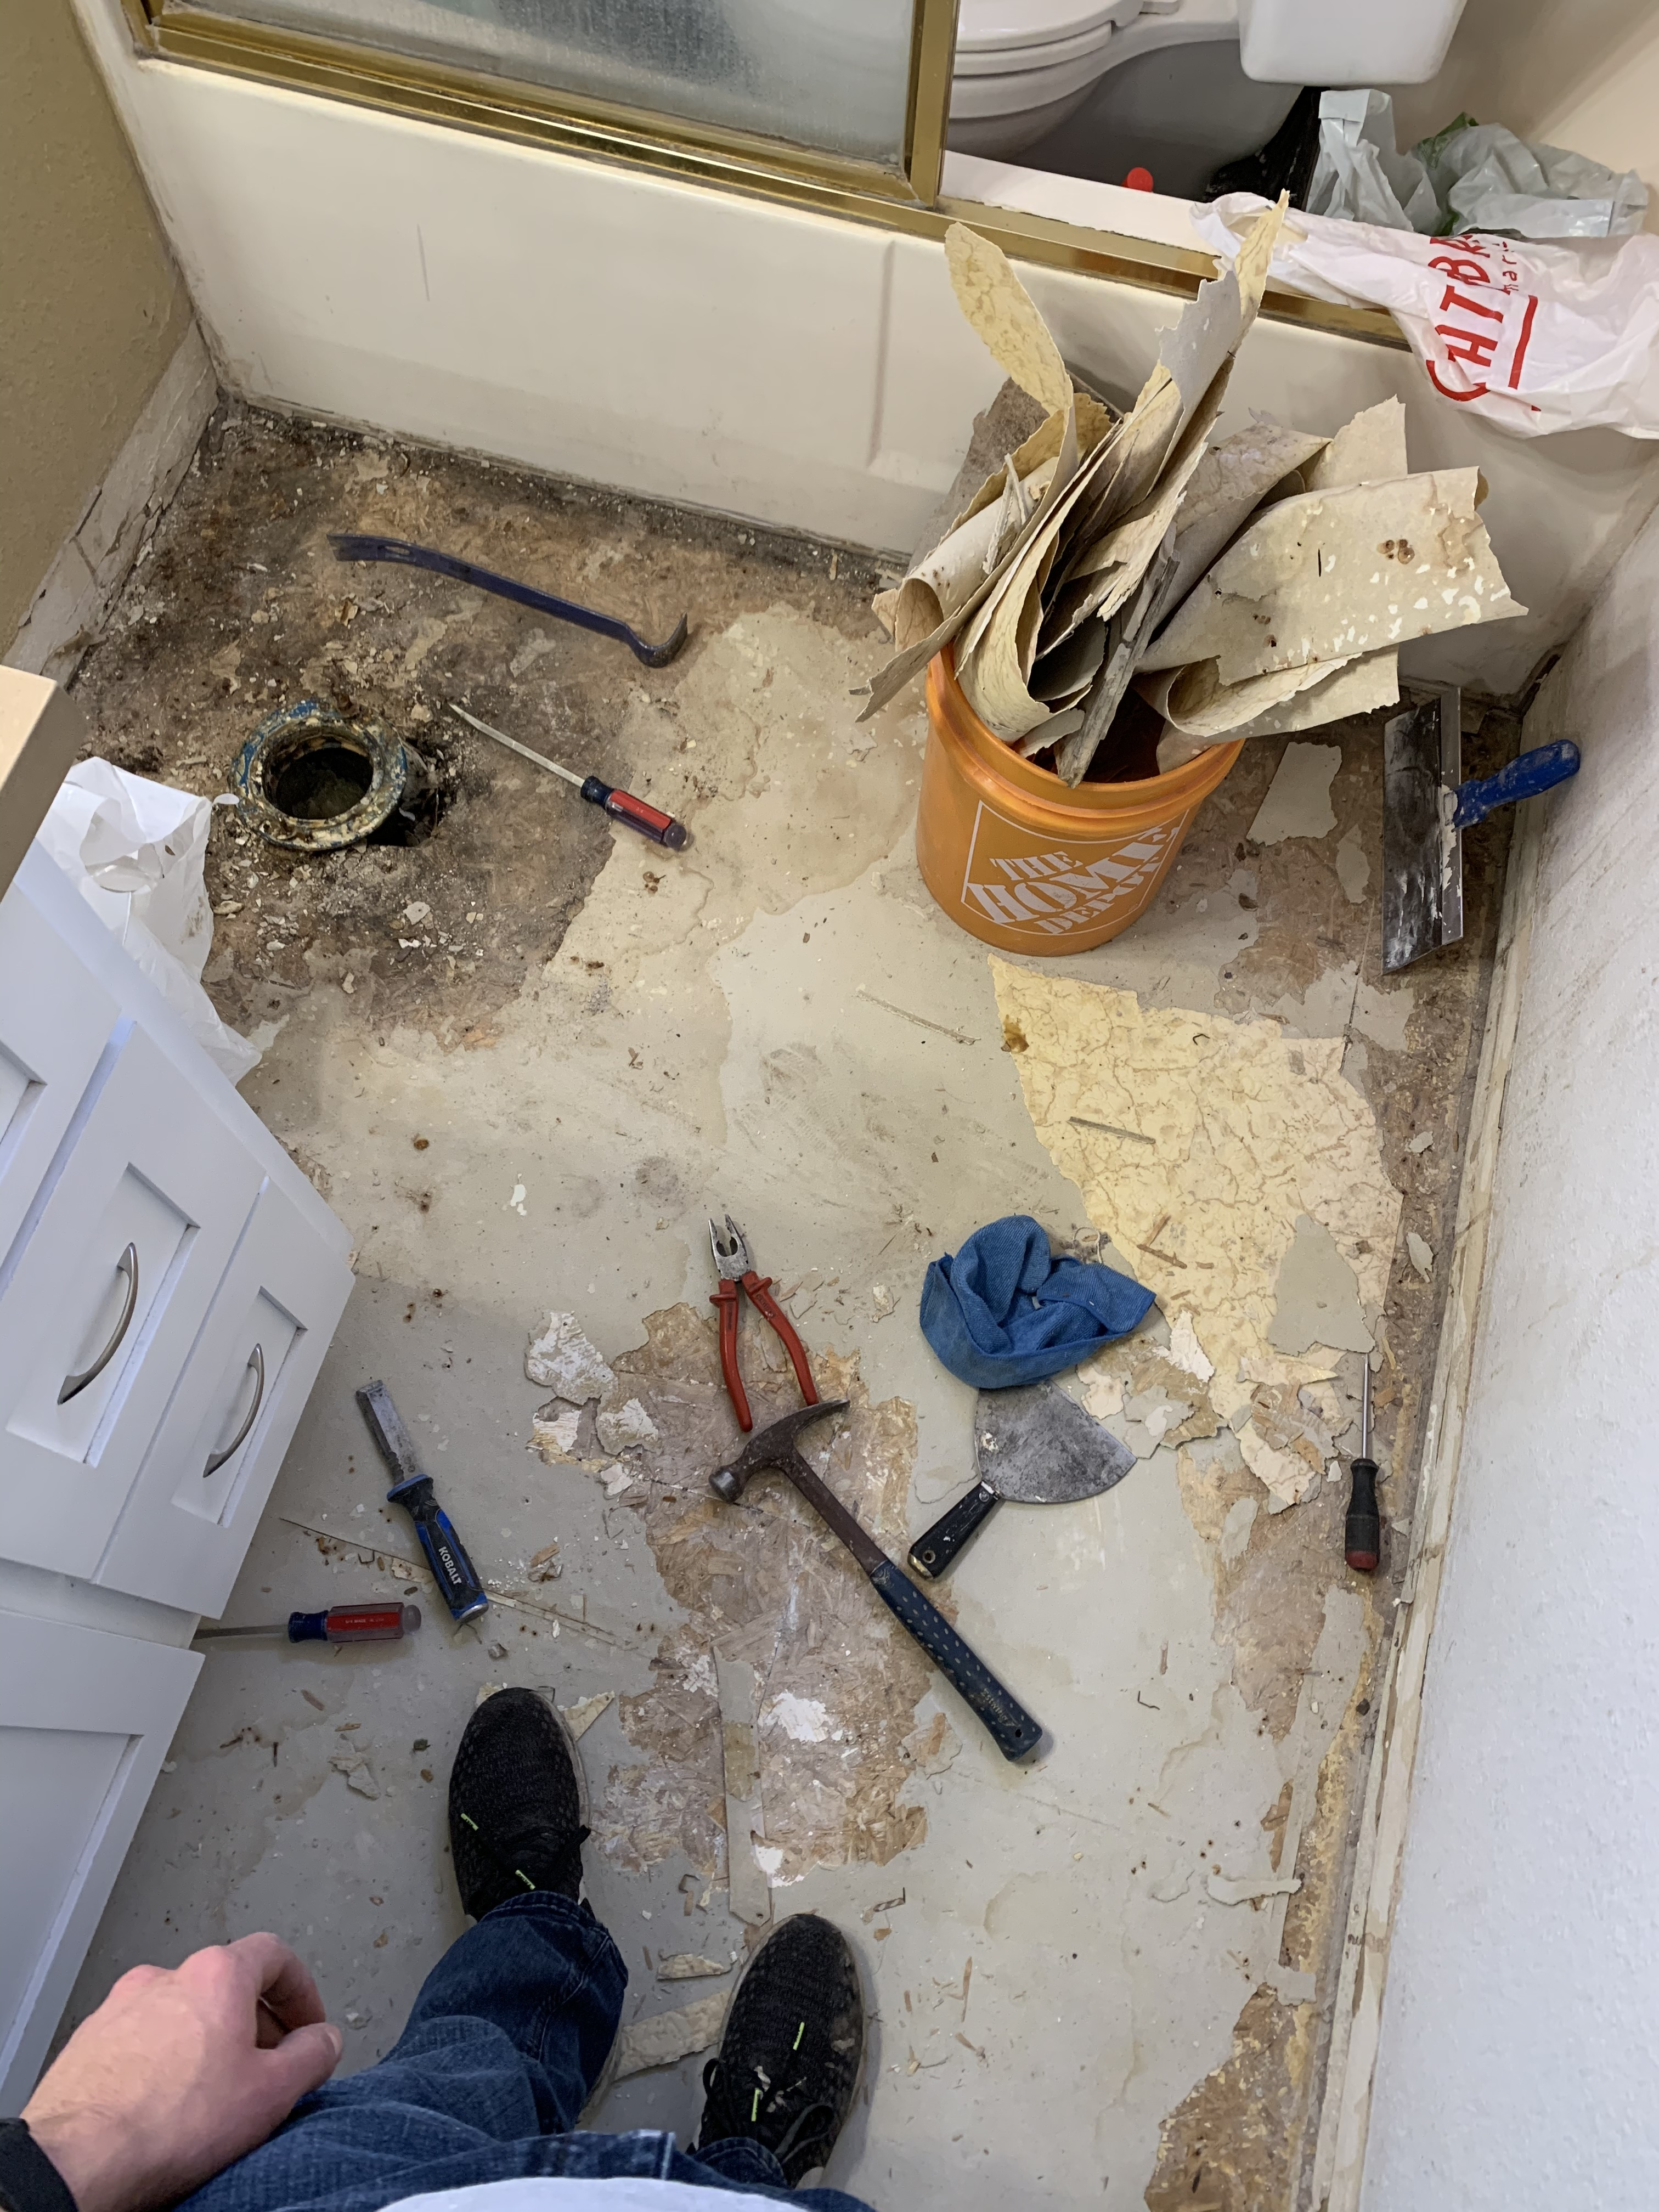
\includegraphics[width=0.6\linewidth]{images/IMG_1769.jpg}
    \caption{Improvised bathroom floor repair using hand tools to remove damaged laminate.}
\end{figure}

This thoughtless act was observed during a bathroom floor repair involving thin laminate flooring designed to resemble tile. The material failed locally near a drain, but its design did not support partial removal or easy repair.

The unmet need was the ability to address localized damage without replacing the entire floor. In response, hand tools were used to manually chip, scrape, and remove sections of the laminate. Tools were spread across the floor, indicating an iterative and improvised repair process rather than a clean, prescribed workflow.

Although labor-intensive, this workaround enabled targeted repair and highlights how materials optimized for installation aesthetics often neglect long-term maintenance. Users adapt their methods to compensate for inflexible design choices when failures occur.

\end{document}